The constant inflow of new experimental measurements 
with unprecedented accuracy from hadron colliders is a remarkable challenge 
for the high energy physics community to provide higher-order theory 
predictions and to develop efficient tools and methods for data analysis.
The recent discovery of the Higgs boson \cite{Aad:2012tfa,Chatrchyan:2012ufa} 
and the extensive searches
for signals of new physics in LHC proton-proton collisions
demand high-precision computations to test the validity of the Standard Model (SM)
and factorisation in Quantum Chromodynamics (QCD).
According to the collinear factorisation in perturbative QCD (pQCD)
hadronic inclusive cross sections are written as
%
%The discovery of the Higgs boson~\cite{Aad:2012tfa,Chatrchyan:2012ufa}
%and extensive searches for signals of new physics at the LHC demands accurate precision of the Standard Model (SM) predictions for
%hard scattering processes in hadron-hadron collisions.
%\\
%The most common approach to calculate the SM cross sections for  
%such reactions is to use collinear factorisation in perturbative QCD (pQCD)~\cite{Collins:1989}:
%{\small
\begin{equation}
\small
\begin{array}{lcl}
\sigma(\as,\mur,\muf) & = &
\sum\limits_{a,b}\,  \int\limits_{0}\limits^{1} dx_1\ dx_2\, f_a(x_1,\as,\muf) 
 f_b(x_2,\as,\muf)\\ 
& \times & \, \hat{\sigma}^{ab}(x_1,x_2;\as,\mur,\muf),
\label{eq:fact}
\end{array}
\end{equation}
%}
where the cross section $\sigma$ for 
any hard-scattering inclusive process
%$ab \rightarrow X + all$
is expressed
as a convolution of Parton Distribution Functions (PDFs) $f_a$ and $f_b$
with the partonic cross section
% that describe
%the 
%$\hat{\sigma}^{ab \rightarrow H + X}$.
$\hat{\sigma}^{ab}$.
%
The PDFs represent 
the probability of finding a specific parton $a$ ($b$) in the first (second) proton carrying a fraction $x_1$ ($x_2$) of its momentum.
%
Indices $a$ and $b$ in the Eq.~\ref{eq:fact} indicate the various 
kinds of partons,
i.e. gluons, quarks and antiquarks of different flavours, 
that are considered
as the constituents of the proton.
%
Both the PDFs and the partonic cross section depend on the strong coupling
$\as$, and the factorisation and renormalisation scales,
$\muf$ and $\mur$, respectively.
%
The partonic cross sections $\hat\sigma^{ab}$ are calculated in pQCD whereas
PDFs are constrained by global fits to variety of the hard-process experimental data employing
universality of PDFs within a particular factorization scheme \cite{Perez:2012um,Forte:2013wc}. 
%
%PDFs are assumed to be universal such that different scattering reactions can be used 
%to constrain them~\cite{Perez:2012um,Forte:2013wc}.
% in particular one can use specific reaction data 
%for determining the PDFs and then use these PDFs for
%predicting other processes.
%

Measurements of the inclusive Neutral Current (NC) and Charged Current (CC)  
Deep-Inelastic-Scattering (DIS) at the $ep$ collider HERA provide crucial information for determining the PDFs.
%
The gluon density in small and medium $x$  
%for calculating the dominant gluon-gluon fusion contribution to Higgs production
%at the LHC 
can be accurately determined solely from the HERA data.
%
Many processes in $pp$ and $p \bar p$ collisions at LHC and Tevatron, respectively, 
probe PDFs in the kinematic ranges, complementary to the DIS measurements.
% (see Fig~\ref{fig:kine}). 
Therefore inclusion of the LHC and Tevatron data in the QCD analysis of the proton structure 
provide additional constraints on the PDFs, improving either their precision, 
or providing valuable information on the correlations of PDFs with the fundamental 
QCD parameters like strong coupling or quark masses. 
%
%\begin{figure}[!ht]
%   \centering
%   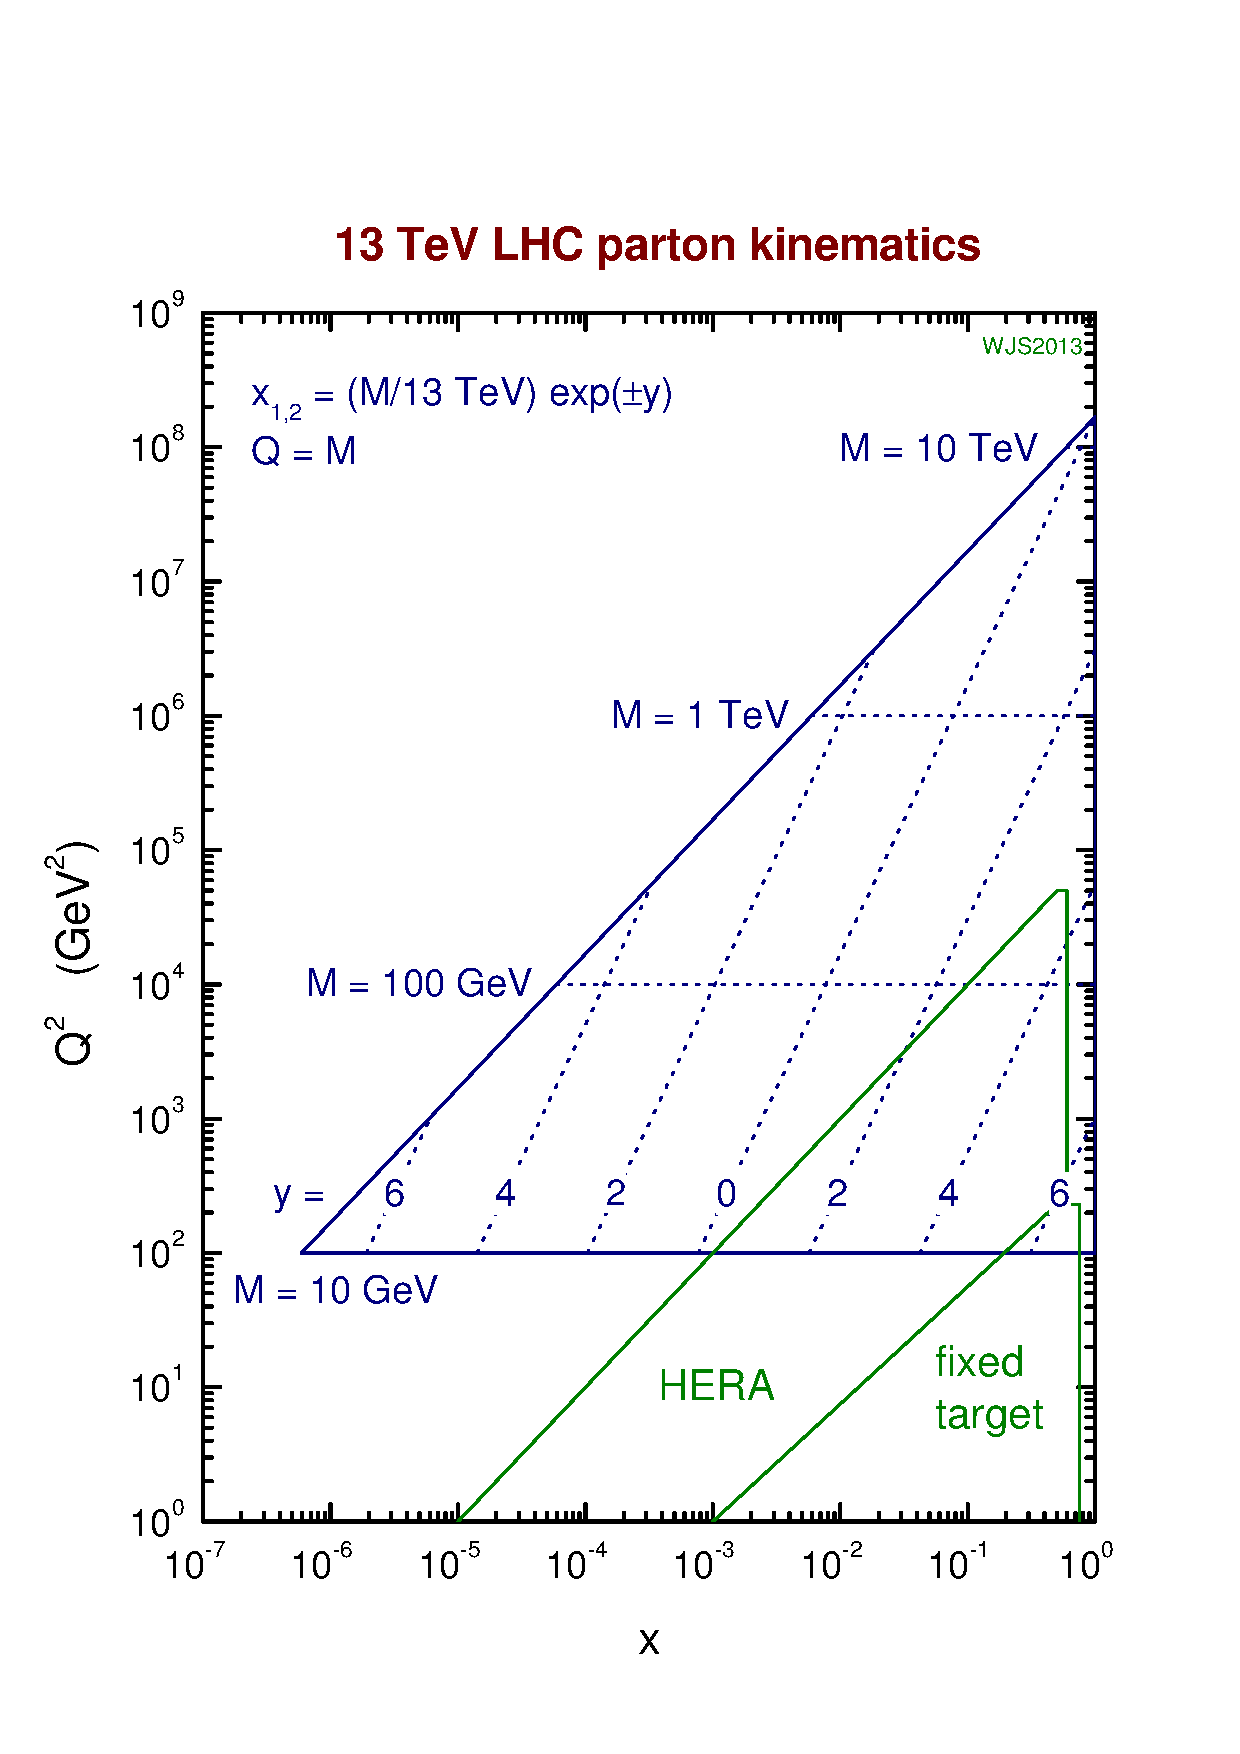
\includegraphics[width=8cm]{kine_stirling.pdf}
%   \caption{The parton kinematic plane with the approximate region sensitivity to the PDFs of LHC and DIS experiments.}
% \label{fig:kine}
%\end{figure}
%%
%Despite being often plagued by larger perturbative uncertainties,
%
In this context, the processes of interest at hadron colliders are
Drell-Yan (DY) production, $W$-boson asymmetries, associated production of $W$ or $Z$ bosons 
and heavy quarks, top quark, jet and prompt photon production.
%

%\fitter~represents a QCD analysis framework that aims at 
%determining precise PDFs by integrating all the PDF sensitive information
%from HERA, the Tevatron and the LHC.
%

This paper describes the open-source QCD platform \fitter which encloses the set of tools  essential for a comprehensive global 
QCD analysis of hadron-induced processes even at the early stage of the experimental measurement. 
It has been developed for determination of PDFs and extraction of fundamental QCD parameters such as the heavy
quark masses or the strong coupling constant. This platform also provides the basis for 
comparisons of different theoretical approaches and can be used for direct tests of the impact 
of new experimental data in the QCD analyses.

This paper is organised as follows.
%
The structure and overview of \fitter are presented in section~\ref{sec:structure}.
Section~\ref{sec:theory} discusses the various processes 
and corresponding theoretical calculations performed in the DGLAP~\cite{Gribov:1972ri,Gribov:1972rt,Lipatov:1974qm,
Dokshitzer:1977sg,Altarelli:1977zs} formalism, available in \fitter.
%
Section~\ref{sec:techniques} presents various fast techniques employed by the theory calculations used in \fitter.
Section~\ref{sec:method} elucidates the 
methodology of determining PDFs through fits based on various
% {\bf (what do you mean here
%by approaches?)} 
 $\chi^2$ definitions used in the
minimisation procedure. 
Alternative approaches to the DGLAP formalism are presented in section~\ref{sec:alternative}.
%
Specific applications of the package are given in
section~\ref{sec:examples} and the summary is presented in section~\ref{sec:summary}.
%
%{\bf add something more here?.}
